
\begin{block}{Related Algorithms}
\begin{itemize}
    \item Prior MMDP algorithms: WSU and MVP
    \item Gradient-based MMDP methods: Mirror and Gradient
    \item Thompson sampling-based algorithms: MixTS
    \item POMDP formulations: QMDP and POMCP
\end{itemize}
% POMDP formulation and MixTS or Thompson sampling
\end{block}


\begin{block}{Simulation Results: Pest Control}
\begin{itemize}
    % \item Initialize $\pi^0$ to the WSU solution and set $\lambda_m, m \in \mathcal{M}$ to be uniform.
    % \item No additional hyper-parameters.
    \item Time horizon $T = 50$, Domain: Pest control simulation
    \item Below figure: mean returns of CADP with different initial policies. 
\end{itemize}
\begin{center}
    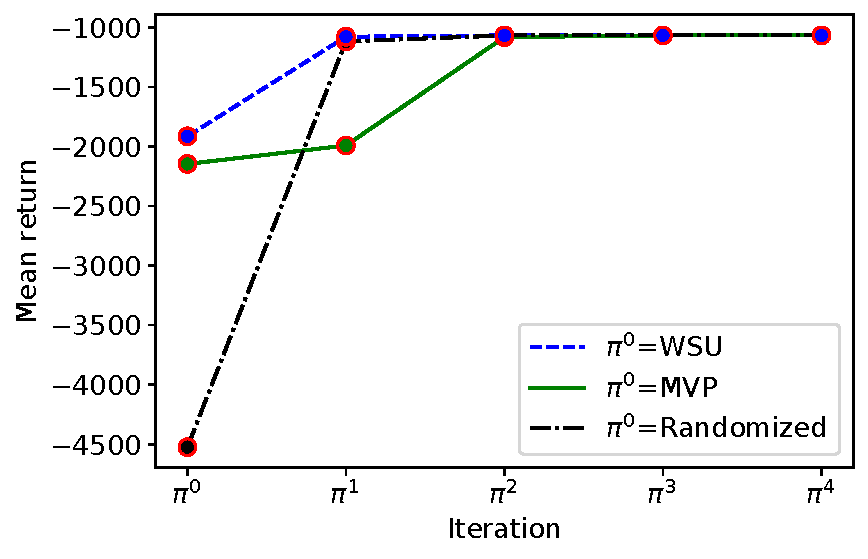
\includegraphics[width=0.6\linewidth]{fig/initial_returns.pdf}
   % Shorter the better
  \end{center}
\begin{itemize}
   \item Left figure: mean returns of algorithms, and right figure: runtimes of algorithms. 
   \item Marker X: no single policy available or runtime is greater than 900 minutes
\end{itemize}
\vspace{0.2cm}
\begin{center}
    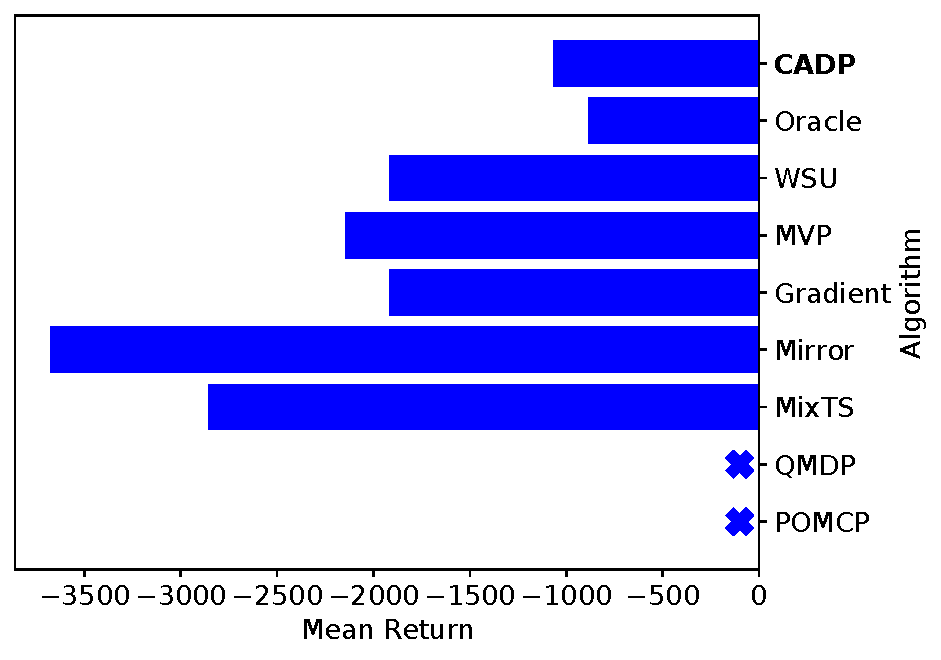
\includegraphics[width=0.49\linewidth]{fig/mean_return.pdf}
    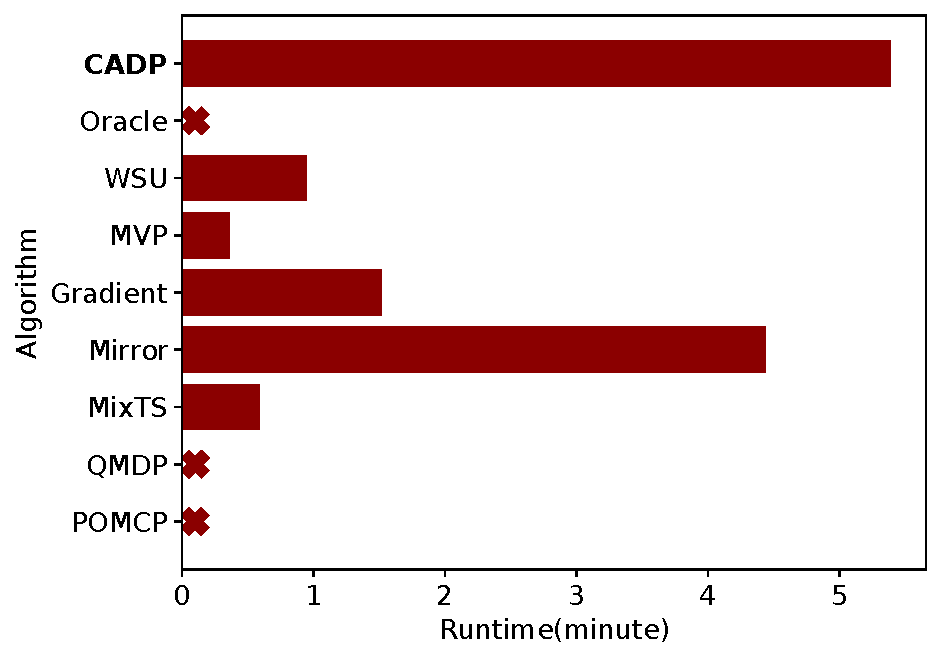
\includegraphics[width=0.49\linewidth]{fig/runtime.pdf}
  \end{center}
\end{block}
\begin{block}{Simulation Results: Other Domains}
\begin{itemize}
    \item Mean returns $\rho(\pi)$ on the test set of policies $\pi$ computed by each algorithm
\end{itemize}

 \begin{table}
    \centering
    \resizebox{\textwidth}{!}{
   \begin{tabular}{lrrrrrrrrrr}
     \toprule
     \textbf{Algorithm}  \bfseries  & \multicolumn{2}{c}{\textbf{RS}} \bfseries & \multicolumn{2}{c}{\textbf{POP}}  \bfseries & \multicolumn{2}{c}{\textbf{POPS}}\bfseries & \multicolumn{2}{c}{\textbf{INV}} & \multicolumn{2}{c}{\textbf{HIV}} \\
     \bfseries   &  T = 50  \bfseries & T =150  &  T = 50  \bfseries & T =150  &  T = 50  \bfseries & T =150  &  T = 50  \bfseries & T =150  &  T = 5  \bfseries & T =20\\
    \midrule
      \textbf{CADP}   &\textbf{204}  & \textbf{207}  & \textbf{-361} &\textbf{-368} &\textbf{-1067} &\textbf{-1082} &323 &\textbf{350} &\textbf{33348} &\textbf{42566}\\
      WSU    &203   &206  &-542     &-551   &-1915 &-1932 &323 &349   &\textbf{33348} &42564\\
      MVP    &201   &204  &-704     &-717   &-2147 &-2179 &323 &\textbf{350}  &\textbf{33348} &42564 \\ 
   \midrule
     Mirror   &181   &183  &-1650    &-1600  &-3676 &-3800 &314 &345   &\textbf{33348} &\textbf{42566}\\
    Gradient   &203   &206  &-542     &-551   &-1915 &-1932 &323 &349   &\textbf{33348} &42564\\
  \midrule
    MixTS      &167   &176  &-1761    &-1711  &-2857 &-3016 &\textbf{327} &\textbf{350}  &293 &-1026\\
    QMDP      &190   &183  & -       &-      &-     &-     &-   &-     &30705  &39626\\ 
   POMCP      &58      & 64    & -       &-      &-     &-     &-   &-     &25794  &30910\\
  \midrule
   Oracle     &210  & 213 &-168     &-172   &-882 &-894  &332 &360   &40159  &53856\\
  \bottomrule
\end{tabular}   
}
\end{table} 
	
\end{block}




